\section{Background}\label{sec:background}

Since the Planner FAPE \citep{bit-monnotFAPEConstraintbasedPlanner2020} is used for the implementation and evaluation, the definitions from \cite{bit-monnotTemporalHierarchicalModels2016a} and \cite{bit-monnotFAPEConstraintbasedPlanner2020} are used as a base throughout the background and approach sections.
The definitions are additionally inspired by \cite{ghallabAutomatedPlanningTheory2004} and \cite{hollerGuidingSearchHTN2019}.
The Planning Domain Definition Language ANML is used to represent the Domain, as it is also used by FAPE.

\subsection{Domain Overcooked}

The application domain is the game "Overcooked" developed by Ghost Town Games and Ltd. and Team 17.
The game models a restaurant kitchen with many simplifications that make the plan abstraction easier and more directly applicable.
The player is given a small number of recipes in each level, for example, a lettuce salad with tomatoes and a burger with a patty, tomatoes and lettuce.
The ingredients often need to be prepared (e.g. by chopping or frying), then arranged on a plate and finally delivered to a conveyor belt that represents the clients.
During playing, fire may break out that has to be extinguished or the players may be separated and can only pass ingredients by placing them on a counter or throwing them to the other cooks for them to prepare or arrange the ingredients.
Additionally, the orders are not known in advance but are received during play and have a strict deadline.
The goal of the game is to successfully finish as many orders as possible; when a deadline is missed it counts as a penalty.
The core part of the game focuses on collaboration and can be played with up to 4 players.
This game is a perfect playground for evaluating and improving planning approaches, as the game poses challenges similar to real life while offering many optional features that challenge the planning domain creation and planning algorithms.
With an appropriate interaction layer, the game may also be used to test acting approaches without the need for a physical robot.
As the game has the option for up to 4 players, the game can be used to evaluate planning for parallel actions when all cooks are supervised by a single planner, or in a multi-agent setting with possible human-robot interaction.
To appropriately fulfill tasks, the agent(s) need to be able to receive tasks during execution.

% The Domain is defined in the DDL Language ANML.
% In the following I will show the most important aspects of the domain that are also considered later.
% The full domain definition is in Appendix 

\subsection{Classical planning}\label{sec:classical-planning}

Classical planning is the widely adopted approach to planning on which most extensions and other planning approaches build upon.
% While there are different ways of representing the problem in classical planning exist, they 
A Planning problem consists of a domain (in our case overcooked) and one or multiple goals e.g. that a client needs to have a burger in the end.
The domain is modeled by creating variables and state transition functions called actions.
The planner is given an initial state and the goal state, and then the planner must find a sequence of actions that can transform the initial state to the goal state.

\begin{definition}[Classical Planning Domain]
  A classical planning domain is a tuple $\Sigma=\langle \mathcal{L}, \mathcal{O}, \delta \rangle$.
  \begin{itemize}
    \item $\mathcal{L}$ is a set of propositional environment variables. 
    \item $\mathcal{O}$ is a set of operator symbols.
    \item $\delta$ is a set $(prec, add, del )$ of functions $f: O \rightarrow 2^L$ that define the state transitions of actions as preconditions and effects.
  \end{itemize}
  An action $a \in O$ is applicable if $\delta(a) \neq \emptyset$.
\end{definition}

The operator symbols contain only action symbols in the case of classical planning.
An action is an expression of the form $a(r_1,\dots,r_n)$ where $a$ is the action symbol and $r_1,\dots,r_n$ are terms (also called parameters).
Constant symbols $D$ are symbols that describe Objects in the domain such as a $Cook$ and are possible instantiations for terms $r$.
Typing is a commonly used extension for planning that organizes constants in the set $L$.
A type $D_t \subseteq D$ restricts variables in actions to be of a specific type such as $Cooks$.
Types can be composed of other types by union or intersection (e.g. $Persons=Cooks\cup Clients$)

\begin{definition}[Classical Planning Problem]
  A classical planning problem is a tuple $P=\langle \Sigma, s_0, g \rangle$.
  $\Sigma$ is a classical planning domain.
  $s_0 \subset L$ is the initial state.
  $g \subset L$ are the goals.
\end{definition}

\subsection{HTN Planning}\label{sec:htn-planning}

Hierarchical Task Network (HTN) planning is a planning paradigm that allows for the specification of complex tasks by the definition of subtasks.
Therefore it is viewed as a control strategy for planning \citep[chap.~11]{ghallabAutomatedPlanningTheory2004}.
Generally, the goal in HTN planning is to decompose complex tasks into primitive executable actions.
% The HTN planning paradigm was first introduced by \cite{erol1994htn} and has since been used in a variety of domains, including robotics \citep{ghallab1998pddl, nau2003shop2, cashmore2008htn, cashmore2015htn}, video games \citep{ontanon2015survey}, and natural language processing \citep{zettlemoyer2005learning, wang2006learning, wang2007learning, wang2008learning, wang2010learning, wang2011learning, wang2012learning, wang2013learning, wang2014learning, wang2015learning, wang2016learning, wang2017learning, wang2018learning, wang2019learning, wang2020learning}.
% HTN Planning can be seen as a guided form of traditional planning, since the task structure is given.


% \cite{hollerGuidingSearchHTN2019}:

A task is an expression of the form $\tau(r_1,\dots,r_n)$ where $\tau$ is a task symbol and $r_1,\dots,r_n$ are the parameters.
There exist primitive tasks where $\tau$ is an action symbol and nonprimitive tasks.

\begin{definition}[Task Network]
  A task network is an acyclic digraph $tn = (T,\prec,\alpha)$ where $T$ is a set of task nodes, $\prec \subseteq T \times T$ is a set of edges that define a strict partial ordering relation between the task nodes and $\alpha: T \rightarrow O$ is a function mapping the task nodes to operator symbols.
\end{definition}

A task network $tn$ is primitive, if all of the task nodes refer to primitive tasks. 

\begin{definition}[HTN Planning Domain]
  An HTN planning domain is a tuple $\Sigma=\langle \mathcal{L}, \mathcal{O}, \mathcal{M}, \delta \rangle$.
  $\mathcal{L},\mathcal{O}$ are defined as in classical planning. 
  $\mathcal{M}$ is a set of methods $(\tau,tn), \tau \in \mathcal{O}$, where $\tau$ is not primitive, that describe possible decompositions from one task into a task network.
  % A task network $tn$ is a triple $(T,\prec,\alpha)$.
  % $\prec \subseteq T \times T$ is a set of strict partial ordering relations between the task identifiers.
  % $\alpha : T \rightarrow A \cup C$ is a function mapping the task identifiers to task or action names.
\end{definition}


\begin{definition}[Task Decomposition]
  A method $m = (\tau,tn)$ decomposes a task network $tn_1 = (T_1,\prec_1,\alpha_1)$ into $tn_2 = (T_2,\prec_2,\alpha_2)$ denoted $tn_1 \xrightarrow{t,m}_D tn_2$, if there is a task node $t_1 \in T_1$ with $\alpha(t_1) = \tau$.
  A copy $tn' = (T',\prec',\alpha')$ of $tn$ is created that has no overlapping task ids with $tn_1$, i.e. $T_1 \cap T' = \emptyset$.
  Then $tn_2$ is defined as:
  \begin{align*}
    tn_2 = & ((T_1 \backslash  \{t\}) \cup T', \prec' \cup \prec_D, (\alpha_1 \ \{t \mapsto c\}) \cup \alpha') \\
    \prec_D = & \{(t_1, t_2) | (t_1, t) \in \prec_1, t_2 \in T'\} \\
    &\cup  \{(t_1, t_2) | (t, t_2) \in \prec_1, t_1 \in T '\} \\
    &\cup  \{(t_1, t_2) | (t_1, t_2) \in \prec_1, t_1 \neq t \land t_2 \neq t\}\\
  \end{align*}
  \label{def:htn-task-dec}
\end{definition}

\begin{definition}[HTN Planning Problem]
  An HTN Planning Problem is defined as a tuple $P=\langle \Sigma, s_0, tn_I \rangle$.
  $s_0 \subset L$ is the initial state.
  $tn_I$ is the initial task network, consisting of the tasks that must be executed.
\end{definition}


% The search through an HTN Planning problem may be done in two conceptually different ways.
% A State-Based Search is the classical approach to solving planning problems.
% A state expansion $f : (L,tn) \rightarrow 2^(L,tn)$ creates a new state for each decomposable task $t$ in the current task network $tn_i$.
% A task is only decomposable if there exists a method $m = (c,tn) \in M$ such that $\delta(m)$
% The planning is finished when all task names in the current task network $tn_i$ are primitive and there is a sequence of the tasks in $tn_i$ that is consistent with its ordering relations.

An important distinction to make is the difference between total order and partial order HTN problems.
In total order problems, $\prec$ is a total order over the tasks, which has double EXPTIME and EXPSPACE-hard complexity.
A partial order problem on the other hand is undecidable \citep{erolHTNPlanningComplexity1994}.


\begin{definition}
  If $tn = (T,\prec,\alpha)$ is primitive, then a plan $\pi = \{a_1,\dots,a_n\}$ is a solution for $P$ if all of the following conditions hold:
  \begin{itemize}
    \item The actions in $\pi$ correspond to the tasks nodes in $T$
    \item $\pi$ is executable in $s_0$
    \item the total ordering $\{a_1,\dots,a_n\}$ satisfies the ordering in $\prec$
    \item the sequence of actions $\{a_1,\dots,a_n\}$ is executable through state transitions from $s_0$
  \end{itemize}
\end{definition}

\begin{algorithm}
  \caption{SHOP}
  \label{alg:background:shop}
  \KwIn{$s$; $tn$; $\Sigma$}
  \KwOut{$\pi$}
  \If{$tn = \varnothing$}{\Return{$\varnothing$}}
  $\tau \leftarrow$ first task in $tn$\;
  $tn' \leftarrow$ remaining tasks in $tn$\;
  \If{$\tau$ is primitive $\land$ there is an action for $\tau$ applicable in $s$}{
    nondeterministically choose an action $a$ for $\tau$\;
    $\pi \leftarrow$ SHOP(apply(s,$a$),$tn'$,$\Sigma$)\;
    \If{$\pi$ = FAIL}{\Return{FAIL}}
    \Return{cons(p,$\pi$)}
  }
  \ElseIf{$\tau$ is not primitive $\land$ there is a decomposition of $\tau$ applicable in $s$}{
    nondeterministically choose a decomposition $m$ of $\tau$ in $s$\;
    $tn \xrightarrow{\tau,m}_D tn'$\;
    \Return{SHOP($s$,$tn'$,$\Sigma$)}
  }
  \Else{\Return{FAIL}}
\end{algorithm}

There are two conceptually different approaches to arriving at a plan $\pi$ for an HTN Planning Problem. 
First, the State-Space approach as in \cite{nauSHOPSimpleHierarchical1999} is shown in algorithm \ref{alg:background:shop}.
The procedure $apply$ applies an action to a state by applying its effects in $\delta$.
Second, the Plan-Space approach as in \citet[sec.~5.4.1]{ghallabAutomatedPlanningTheory2004} is shown in algorithm \ref{alg:background:psp}.
There a partial plan is used, that is created by resolving flaws.
A flaw in HTN planning may be an unrefined task or a possible inconsistency.
A resolver is a modification of a partial plan and task network, that is applied using the procedure Transform.
The internal representation of $\delta$ in Plan-Space planning is often done using Constraint Satisfaction instead of direct manipulation of states.

\begin{algorithm}
  \caption{PSP}
  \label{alg:background:psp}
  \KwIn{$\pi$; $tn$; $\Sigma$}
  \KwOut{$\pi$}
  Flaws $\leftarrow$ flaws in $\pi$\;
  \If{Flaws = $\varnothing$}{\Return{$\pi$}}
  $\varphi \leftarrow$ select a flaw in Flaws\;
  Resolvers $\leftarrow$ resolvers for $\varphi$\;
  \If{Resolvers = $\varnothing$}{\Return{FAIL}}
  nondeterministically choose $\rho \in Resolvers$\;
  $(tn',\pi') \leftarrow \text{Transform}((tn,\pi), \rho)$\;
  \Return{$\text{PSP}((tn',\pi'); \Sigma)$}
\end{algorithm}



% To create $\pi$ the HTN Planning Problem is formulated as a search.
% The search may be done in two different ways.
% State-Based Planning is similar to the classical approach of solving planning problems.
% The alternative is Plan-Space Planning which uses Flaws and Resolvers.
% In this case, the constraints defined by $\delta$ and $M$ are added to a dynamic CSP.
% The current Search node is called a Partial Plan $\hat{\pi}$, and may contain Flaws.
% If there are no Flaws left and the CSP is consistent, then $\hat{\pi}_i = \pi$.
% A Flaw can be one of:
% \begin{itemize}
%   \item Threat: There is a potential inconsistency in the CSP
%   \item UnboundVariable: The domain of a variable in the CSP contains more than one value. This occurs when there are multiple possible instantiations of a task, method or action.
%   \item UnmotivatedAction: An action is not part of a task decomposition. This may happend when a task is removed from the network during replanning.
%   \item UnrefinedTask: A task is not yet decomposed.
% \end{itemize}

% HTN Planning problems can be defined in several languages, such as the SHOP syntax, supported by SHOP-Like planners, ANML Language - supported by the FAPE planner and HDDL Syntax which is expected to become the standard.
% While these languages mostly support the same features, it is important to note that HDDL currently only supports a small subset of the PDDL syntax it is based on, primarily because the most HTN planners do not support temporal or resource planning.
% The HDDL 2.1 proposal adds the support for Temporal planning, but there is currently no public system that supports this syntax.
% The most expressive Syntax is the ANML-Language, which also supports dynamic fluents that change over time.
% This Syntax is used throughout the whole thesis, as it supports Time for HTN Planning and is much less verbose than SHOP.
% The FAPE planner is therefore used as a basis for this work.

\subsubsection{Temporal HTN Planning}\label{sec:temporal-htn-planning}

Temporal HTN Planning includes explicit information about time in the domain.
This allows modeling task durations, concurrent execution, start points and deadlines for tasks.
CSP Encodings of the planning problem are a popular strategy and makes even more sense here.
\cite{stockHierarchicalHybridPlanning2015} introduced the notion of a MetaCSP, that solves two constraint satisfaction problems, the normal CSP for variable constraint, and a Temporal Network managing the temporal constraints over time points.
This approach is also used in FAPE.
The main components required to model the Temporal HTN Planning Problem are introduced in the following paragraphs. 


Time is represented quantitatively using time points. % as in Simple Temporal Networks (STempN)  \citep{dechterTemporalConstraintNetworks1991}.
A time point is designated by a temporal variable (e.g. $t_1$).
Constraints over temporal variables can be expressed using the simple arithmetic operators $=,\leq,\geq$ to specify absolute  (e.g. $t_1 \geq 10$) or relative constraints (e.g. $t_1 + 5 \leq t_2$).
The temporal variables are attached to events like the start of an action or an instant at which a condition must hold.

A nontemporal variable $c \in D_t$ is a variable with a domain $dom(c) \subseteq D_t$.
A numeric variable $i$ has a domain $dom(i) \subset \mathbb{N}$ which is a finite subset of integers.
A constraint over a set of variables $\{v_1,\dots ,v_n \}$ is a pair $(\langle v_1, \dots, v_n \rangle, \gamma_R)$ where $\gamma_R \subseteq dom(v_1) \times \dots \times dom(v_n)$ is the relation of the constraint, giving the allowed values for the tuple of variables.
$\gamma_R$ can be given as a table of allowed values or a function, e.g., $\textit{distance}(d, d') = \Delta$ is met when $\Delta$ is the distance between $d$ and $d'$.
Numeric variables can also appear in temporal constraints.
For instance $(\textit{distance}(d, d') = \Delta) \land (t_s + \Delta \leq t_e)$ describes a constraint that defines that the delay between $t_s$ and $t_e$ is equal to the distance $\Delta$ between $d$ and $d'$.
This constraint may occur as the duration of an action $move(d,d')$, with time points $t_s$ as the actions start and $t_e$ as the actions end.

\begin{definition}[State Variable]
  An n-ary state variable $sv(v_1,...,v_n)$ is a function $x: time \times D_1^x \times \dots \times D_n^x \rightarrow D_{n+1}^x$ that maps time and a set of variables to a variable.
  Each $D_i^x \subseteq D$ is the union of one or more types.
  Time in a state variable is usually kept implicit and we say that $sv$ has the value $v$ at time $t$ if $sv(t,x_1,...,x_n) = v$.
\end{definition}

State variables are a convenient way to describe the change of a variable over time as a function of that variable over time.
For instance $Ingredient.location: Time \times \textit{Ingredients} \rightarrow \textit{ Persons } \cup \textit{ Placement Areas } \cup \textit{ Tablewares }$ specifies the location of any ingredient at any point in time, which may be in a person's hand, in an area or on a tableware.
Complete knowledge about the value of each variable is not required for planning.

\begin{definition}[Fluent]
  A fluent is a pair of a state variable $sv$ and a value $v$, denoted $\langle sv=v \rangle$ and is said to hold at time $t$ if $sv$ has the value $v$ at time $t$.
\end{definition}

A fluent $Ingredient.location(lettuce1) = cook1$ may then hold at several points in time, for example between $cook1$ picking it up and $cook1$ placing it on a plate.
Fluents are used to define and are extended by temporally qualified assertions:

\begin{definition}[Temporally qualified assertions]
  A temporally qualified assertion $\alpha$ is an assertion over a state variable $sv$ in a temporal interval $[t_s,t_e]$.
  The temporal interval may also describe an instant $t$ denoted as $[t]$.\\
  A persistence assertion, denoted $\alpha = \langle [t_s,t_e] sv=v \rangle$, requires $sv$ to keep the same value $v$ over the temporal interval $t_s,t_e$.\\
  A change assertion, denoted $\alpha = \langle [t_s,t_e] sv : v_1 \mapsto v_2 \rangle$ describes that $sv$ changes its value from $v_1$ at time $t_s$ to $v_2$ at time $t_e$. \\
  A temporally qualified assignment denoted $\alpha = \langle [t] sv := v \rangle$ describes that $sv$ has the value $v$ at time $t$.
\end{definition}

Persistence assertions are typically used to express requirements such as goals or pre-conditions of actions.
For instance $\langle[100,200] loc(lettuce1) = counter1\rangle$ requires the instance $lettuce1$ to be at the location $counter1$ from time 100 until time 200.
The change assertion is typically used to combine pre and post-conditions of most planners into one and additionally to explicitly describe the value change as a process rather than an instantaneous effect.
For instance, $\langle [100,200] chopped(lettuce1) : false \mapsto true \rangle$ describes that the instance $lettuce1$ is getting chopped from time 100 until time 200.
An assignment is a special case of a change assertion $\alpha = \langle [t-1,t] sv: any \mapsto v \rangle$ where $any$ is a variable with a possibly infinite domain.
For instance $\langle [0] chopped(lettuce1) := false \rangle$ states that the instance $lettuce1$ is not chopped at time 0.

State variables are a replacement for the propositional variables $\mathcal{L}$ and therefore also states.
They make time explicit and move change states along individual variables instead of globally.
They offer a more compact representation and higher expressivity than propositional variables.
Additionally, it is now implicitly defined that an object can only be in one place at any time, which has to be done using external domain constraints in classical representations. 
Lastly, they do not have to be the result of an action but value changes can be predefined at any time interval.

\begin{definition}[Timeline]
  A timeline is a pair $(\mathcal{F},\mathcal{C})$ where $\mathcal{F}$ is a set of temporally qualified assertions on a state variable and $\mathcal{C}$ is a set of constraints on objects and temporal variables appearing in $\mathcal{F}$.
\end{definition}
A timeline describes a partial evolution of the state variable over time.
It is only partial because the timeline is supposed to be consistent in itself.
Due to the inconsistent states while planning, several timelines for a single state variable for a partial plan may exist during planning, but they must be combined at the end.
For the details on consistency, see \cite{bit-monnotTemporalHierarchicalModels2016a}.


\begin{definition}[Chronicle]
  A chronicle is a triple $\phi = (\pi,\mathcal{F},\mathcal{C})$ where $\pi$ is a partial plan composed of action instances and unrefined tasks and $(\mathcal{F},\mathcal{C})$ is a set of timelines.
\end{definition}
The chronicle in \cite{bit-monnotFAPEConstraintbasedPlanner2020} is a temporal and hierarchical extension of partial plans in plan-space planning approaches \citep[chap.~5]{ghallabAutomatedPlanningTheory2004} and extends the notion of chronicles in \cite[sec.~4.2.4]{ghallabAutomatedPlanningActing2016} with the member $\pi$ to keep track of tasks and actions.

% Tasks and Actions are defined slightly different in FAPE compared to other literature, but behave equivalent.
% While there are no Methods, an Action with subtasks is equivalent to a method.
% An Action Template defines the properties of an Action.

Tasks, Methods and Actions are defined differently in FAPE compared to the common HTN Approach.
Action Templates combine the notion of an Action and a Method.
Tasks $\mathcal{T}$ are no longer split between primitive and non-primitive tasks.
\cite{bit-monnotTemporalHierarchicalModels2016a} argues that the distinction between primitive and nonprimitive tasks as well as Actions and Methods is only an artificial restriction and that it has no impact on the planning implementation.

\begin{definition}[Action Template]
  An action template is a tuple \\ $(head(A), task(A), dependent(A), subtasks(A), \mathcal{F}_A, \mathcal{C}_A)$ where
  \begin{itemize}
    \item $head(A) = a(r_1,\dots,r_n)$ is the action symbol $a$ and the parameters $r_1,\dots,r_n$ of $A$.
    \item $task(A) \in \mathcal{T}$ is the task $\tau(r_1,\dots,r_n)$ that $A$ achieves.
    \item $dependent(A) \in \{\top,\bot\}$ defines if $A$ is task dependent, meaning if an action $a$ fulfilling $A$ can only be inserted if a $task(A)$ is achieved through $a$.
    \item $subtasks(A)$ is a set of temporally qualified subtasks written as $\langle[t_s,t_e] \tau\rangle$.
    \item $(\mathcal{F}_A, \mathcal{C}_A)$ is a consistent set of timelines.
  \end{itemize}
\end{definition}

The start and end time points of the action template and the subtasks are all left implicit.
An action template is high-level, if $subtasks(A) \neq \varnothing$, otherwise it is primitive.
A method $(c,tn)$ is part of a high-level action template through $subtasks(A)$ and $\mathcal{C}_A$.
A task is primitive, if there is only one action template $A$ that achieves it and that action template is primitive.

\begin{definition}[Task Decomposition in FAPE]
  A chronicle $\phi_1 = (\pi_1,\mathcal{F}_1,\mathcal{C}_1)$ can be refined into a chronicle $\phi_2 = (\pi_2,\mathcal{F}_2,\mathcal{C}_2)$ by decomposing an unrefined task $\tau \in \pi_1$ with a new action instance $a$. This transformation is denoted $\phi_1 \xrightarrow{\tau,a}_D \phi_2$ and does the following modifications to $\phi_2$
  \begin{align*}
    \pi_2 \leftarrow & \pi_1 \cup \{a\} \cup subtasks(a) \backslash \{\tau\} \\
    \mathcal{F}_2 \leftarrow & \mathcal{F}_1 \cup \mathcal{F}_a \\
    \mathcal{C}_2 \leftarrow & \mathcal{C}_1 \cup \mathcal{C}_a \cup \{task(a) = \tau\} \\
  \end{align*}
  \label{def:htn-task-dec-fape}
\end{definition}

This decomposition definition is much more straightforward than \ref{def:htn-task-dec}, as it leaves the burden of constraint solving on the MetaCSP.
The additional constraint $\{task(a) = \tau\}$ ensures that $a$ does refine $\tau$ correctly by unifying the parameters and time points of $a$ and $\tau$.

\begin{definition}[Temporal HTN Planning Domain]
  A temporal HTN planning domain is a tuple $\Sigma = \langle \mathcal{SV},\mathcal{O},\mathcal{A} \rangle$.
  $\mathcal{O}$ is defined equivalently to the standard HTN Planning Domain.
  $\mathcal{SV}$ is a set of state variables.
  $\mathcal{A}$ is a set of action templates.
\end{definition}

\begin{definition}[Temporal HTN Planning Problem]
  A temporal HTN planning problem is a pair $P = \langle \Sigma, \phi_0 \rangle$.
  $\Sigma$ is a temporal HTN planning domain.
  $\phi_0$ is the initial chronicle.
\end{definition}

While the definitions for Temporal HTN Planning in FAPE are quite different from HTN Planning, fundamentally it is very similar.
A chronicle $\phi$ is a temporal extension of a task network $\langle T,\prec,\alpha \rangle$.
The tasks $T$ are contained in $\pi$ and $\prec$ is contained in the constraints $\mathcal{C}$.
$\alpha$ does not exist anymore, but the mapping from actions and tasks to their names is similar.


\begin{definition}[Temporal HTN Planning Solution]
  $\phi = (\pi,\mathcal{F},\mathcal{C})$ is a solution for $P$ if all of the following conditions hold:
  \begin{itemize}
    \item $\phi$ is reachable from $\phi_0$.
    \item $\pi$ does not include tasks.
    \item all assertions in $\mathcal{F}$ are causally supported.
    \item $(\mathcal{F},\mathcal{C})$ is a set of necessarily consistent timelines.
  \end{itemize}
\end{definition}

In temporal HTN planning, it is infeasible to use a State-Space Planning approach as actions might be required to be parallel and State-Space Planning cannot insert several actions at once.
Therefore FAPE uses Plan-Space Planning as in algorithm \ref{alg:background:psp}.

\subsubsection{Task insertion}

HTN Planning with task insertion is a formalism that lies between classical planning and HTN planning.
The idea here is to allow the insertion of tasks into the task network during planning, without requiring them to be valid decompositions of compound tasks.
This approach is helpful for example in domains where not all possible hierarchical tasks can be captured, and allows an agent to respond to unforeseen situations.
Additionally, it allows the usage of heuristics used in classical planning in combination with heuristics in HTN Planning.

FAPE supports task insertion directly, however there it is called action insertion.
The initial chronicle can define persistence assertions as the goals a planner needs to achieve.
Tasks can be marked as insertable if it is not marked $dependent$ in the action template definition.
There is then a separate plan modification called Action Insertion to add the action to the chronicle $\phi$ that is very similar to definition \ref{def:htn-task-dec-fape}:

\begin{definition}[Action Insertion]
  A chronicle $\phi_1 = (\pi_1,\mathcal{F}_1,\mathcal{C}_1)$ can be refined into a chronicle $\phi_2 = (\pi_2,\mathcal{F}_2,\mathcal{C}_2)$ by inserting a free action instance $a$, i.e. $a$ is not task-dependent. This transformation is denoted $\phi_1 \xrightarrow{a}_I \phi_2$ and does the following modifications to $\phi_2$
  \begin{align*}
    \pi_2 \leftarrow & \pi_1 \cup \{a\} \cup subtasks(a) \\
    \mathcal{F}_2 \leftarrow & \mathcal{F}_1 \cup \mathcal{F}_a \\
    \mathcal{C}_2 \leftarrow & \mathcal{C}_1 \cup \mathcal{C}_a \\
  \end{align*}
\end{definition}

The distinction between task insertion and action insertion is important since the insertion of a task allows the decomposition into multiple different actions.
Additionally, it is easier to evaluate if it is possible to insert an action than a task, since tasks do not have any constraints that can be used for validation.




\subsection{Online Planning and Acting}\label{sec:acting}

% Where to put the Stream?
\begin{figure}
  \centering
  \subfloat[With generic deliberation function]{\label{fig:background-acting-conceptual-deliberation}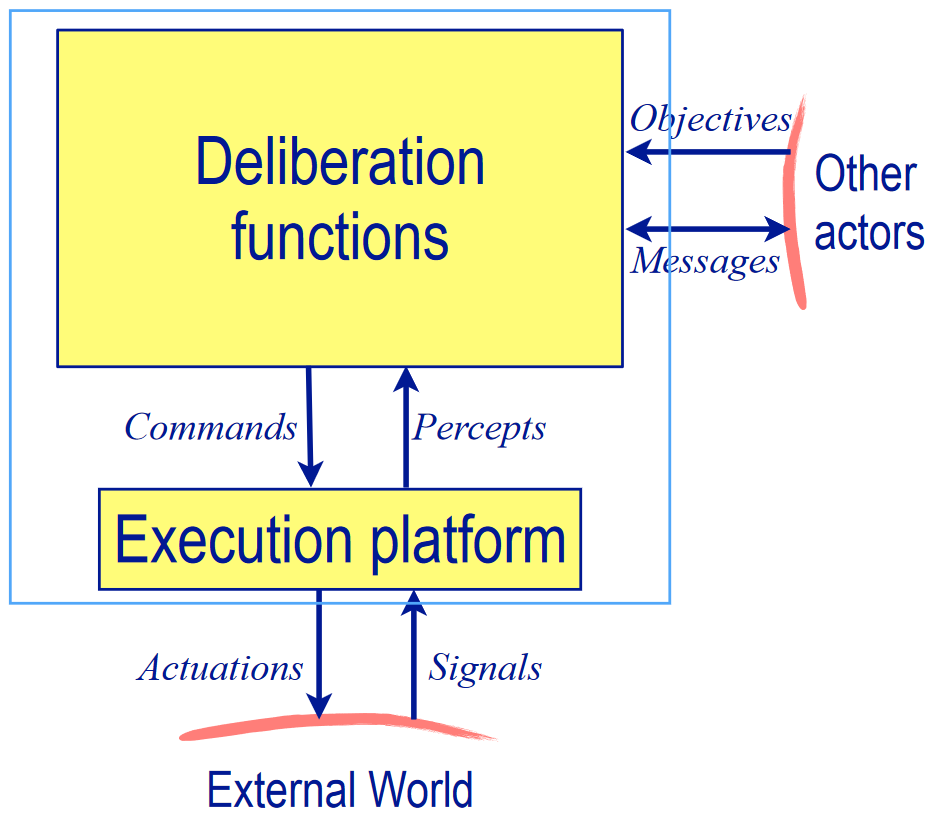
\includegraphics[width=0.4\textwidth]{images/background_acting_conceptual_deliberation.png}}
  \subfloat[With only planning and acting]{\label{fig:background-acting-conceptual-pa}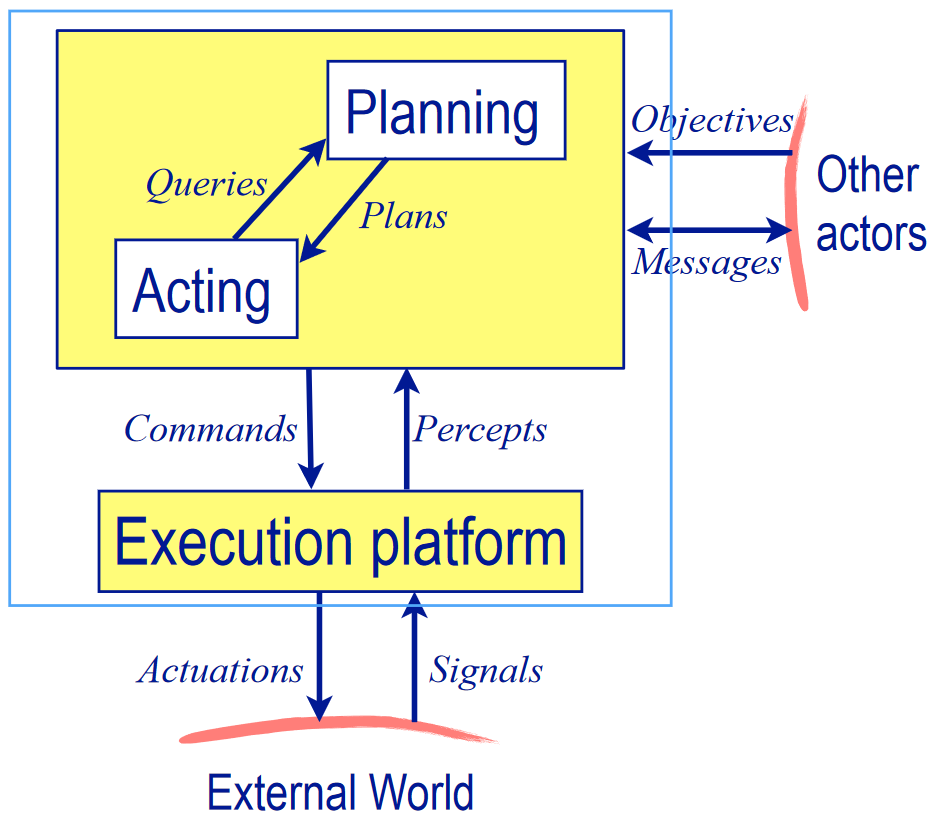
\includegraphics[width=0.4\textwidth]{images/background_acting_conceptual_p_a.png}}
  \caption[Conceptual view of an actor]{Conceptual view of an actor from \cite{ghallabAutomatedPlanningActing2016}}
  \label{fig:background-acting-conceptual}
\end{figure}

The offline planning approach described in the previous sections does not yet describe, how the plan will be executed in an environment like the Overcooked Game and what happens if new tasks are received.
In \cite{ghallabAutomatedPlanningActing2016} an Actor is described as a system that uses deliberation functions and an execution platform to interact with the external environment and other actors.
In particular, deliberation functions describe an interaction between Acting, Planning and other deliberation functions such as Observing, Monitoring, Goal reasoning and Learning \citep{ingrandDeliberationAutonomousRobots2017} (see figure \ref{fig:background-acting-conceptual}).
Directly relevant for this use case are only Acting and Planning.




Acting is then defined as the decision on how to perform actions given by a planner, considering the current state of the observed environment.
It also involves reacting to unexpected states and triggering plan repairs or replanning in the online planning algorithm.
Such an unexpected state is in our case the addition of new tasks during execution.

The actor architecture of FAPE (see figure \ref{fig:background-acting-fape}) implements this general model.
The Activity Manager takes the role of both Acting and State Management and requests the Planner for updates.
The Skills are concrete implementations of action executions that are selected by the Activity Manager.
The Observation Database tracks changes in the environment and informs the Activity Manager that needs to decide if plan repair is necessary.


\bild{fig:background-acting-fape}{background_acting_fape}{General architecture of FAPE for online planning and acting}{10}



Online planning is an algorithm that can update and refine a plan when a plan modification occurs.
A plan modification in this case can be a failed action that has to be removed, a change in the environment or a new task.
Online planning in HTN has to take the already executed actions and hierarchy into account.
There are 2 possible procedures:
\begin{itemize}
  \item Replanning: Remove all pending actions and find an alternative plan.
  \item Plan Repair: Remove the smallest set of problematic actions and find alternative decompositions.
  % \item Partial Decomposition: Only decompose tasks when they need to be executed.
\end{itemize}

While all of these procedures will arrive at a successful plan if it exists, the complexities vary.
Replanning is the simplest approach where only a new plan search is executed.
Plan Repair is often implemented as a local search around conflicting actions, which introduces another complex problem.
In the worst case, Plan Repair equals Replanning in the Result but not in Complexity.
However, Plan Repair has better plan stability \citep{foxPlanStabilityReplanning2006}.
% Partial Decomposition has only 

% The initial versions of online planning for classical planning describe it as the generation of partial plans through subgoaling, limited horizon planning or sampling \citep{ghallabAutomatedPlanningActing2016}.

% However, in the context of temporal HTN problems, partial solutions are not feasible as the plan-space planning does not directly allow for partial solutions.
% Thus online planning is defined as the possibility of a planner to repair or replan.


% \missingfigure[]{Planning procedure?}

% If there is no inconsistency, the plan search can be executed directly.
% If planning fails like this, replanning is done.
% Plan Repair is done by removing conflicting actions and then executing the plan search.
% If Repair fails, replanning is done.
% Replanning is done by removing all pending actions and conflicting actions and then executing plan search.

% describes that a planner can receive updates  and through acting plans are executed in a real world environment.
% The challenges here include uncertainty in the environment, failure of actions and therefore replanning, and the need for real-time performance.
% Replanning with HTN Planning is another challenge, since the hierarchy of tasks must be considered and replanning cannot be done trivially.


% There are different approaches to preforming acting, depending on the uncertainties in the environment.
% In the most uncertain environments, lookahead planning is common, where only a few of the upcoming steps are used to guide the search. 
% On each new state the planning is repeated.
% When the environment has more certainty, the planning is executed fully and the plan is followed until a state occurs that differs from the state predicted by the planner.
% Then it is attempted to repair the plan. 
% If that does not work, a full replanning is done.

% There are different approaches to Plan Repair, the most prominent are to remove 

% Acting with a HTN Planner can be done similar, but requires more care, since the hierarchy does not enable a direct replanning.
% \cite{desilvaHTNActingFormalism2018} has introduced a formalism and algorithm for HTN acting that contains the following steps:
% A configuration represents the current state of the planning.
% Primary Tasks are the tasks that can be executed, which requires that there are no tasks that precede them.
% There are different possibilities for execution:
% Execution via reduction: A task is executed when it is reduced/decomposed using a method body
% Execution via performing an action: A (primary) action can be executed if it is applicable.
% Execution via replacement: A method body

% Most of the approaches for do not cover the case of new targets explicitly, as it may be handled directly by the repair and replan approach.
% The only reference that touched on this case is \cite{desilvaHTNActingFormalism2018}.
% They introduced an algorithm where it was possible to add tasks at any point during acting.
% These tasks may also describe environment changes, that may be the triggers for replanning.


